% Hamming trust regions of radius 1 and 2 around the incumbent (7,6),
% ten subdivisions per variable.
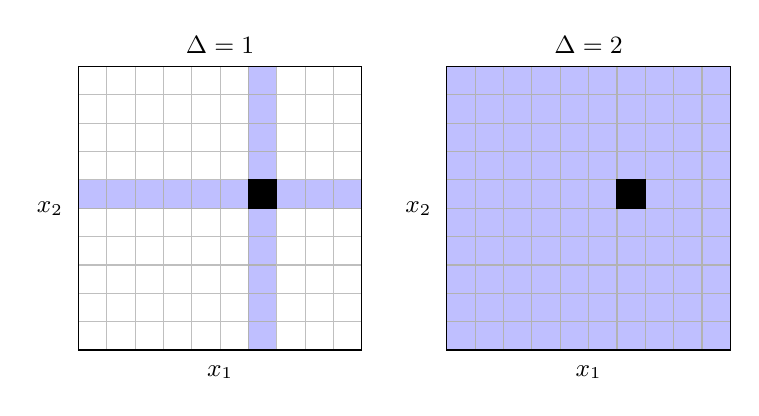
\begin{tikzpicture}[x=0.36cm,y=0.36cm,font=\small]
  \foreach \panel/\radius/\shift in {a/1/0, b/2/13}{
    \begin{scope}[xshift=\shift cm*0.36]
      \foreach \i in {1,...,10}{
        \foreach \j in {1,...,10}{
          \pgfmathtruncatemacro{\changed}{(\i!=7)+(\j!=6)}
          \ifnum\changed>\radius\relax
            \draw[gray!50,fill=white] (\i-1,\j-1) rectangle ++(1,1);
          \else
            \draw[gray!60,fill=blue!25] (\i-1,\j-1) rectangle ++(1,1);
          \fi
        }
      }
      \draw[fill=black] (6,5) rectangle ++(1,1);
      \draw (0,0) rectangle (10,10);
      \node[below] at (5,-0.2) {$x_1$};
      \node[left] at (-0.2,5) {$x_2$};
      \node[above] at (5,10.1) {$\Delta = \radius$};
    \end{scope}
  }
\end{tikzpicture}
